% @Author: AnthonyKenny98
% @Date:   2020-02-27 14:22:10
% @Last Modified by:   AnthonyKenny98
% @Last Modified time: 2020-04-03 14:28:31

\begin{figure}[H]
\begin{center}
\begin{tabular}{c c}

    % Subfigure A
    \begin{subfigure}{0.45\textwidth}
    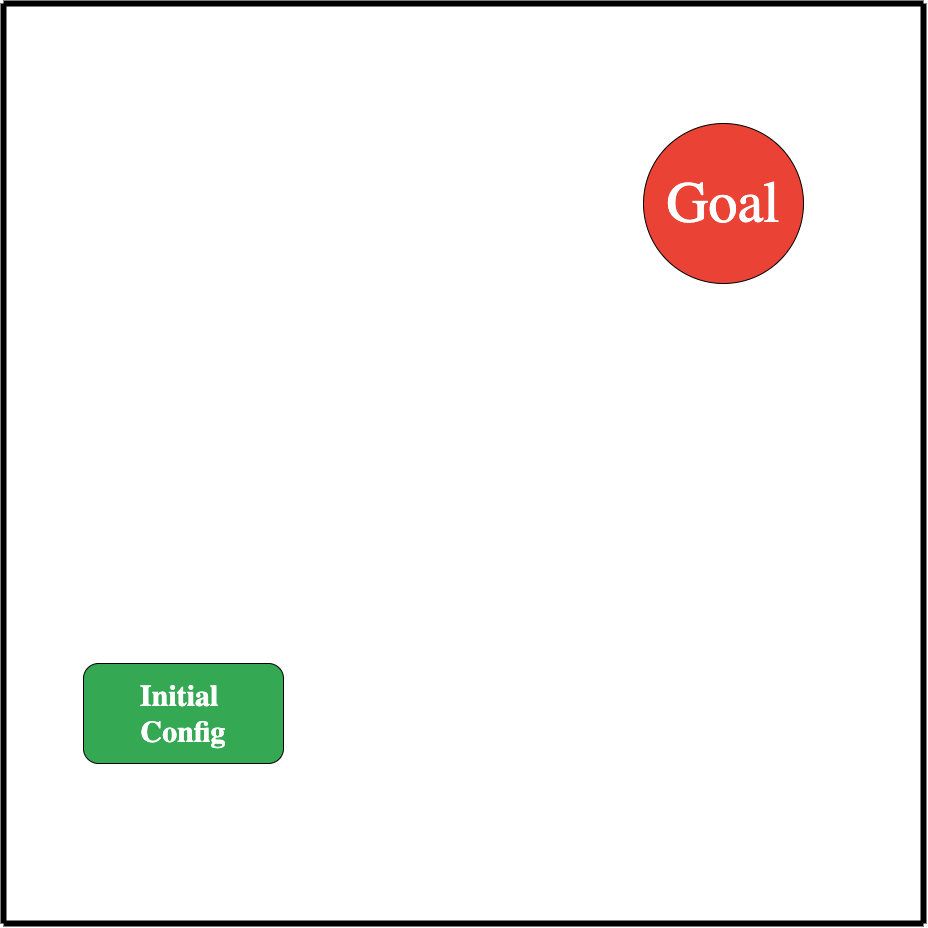
\includegraphics[width=\linewidth]{chapters/chapter2/img/RRT_step_by_step-A.png}
    \caption{Graph $G$ contains only $q_{init}$ \newline}
    \label{subfig:rrt-step-by-step-A}
    \end{subfigure} &
    % 
    % Subfigure B
    \begin{subfigure}{0.45\textwidth}
    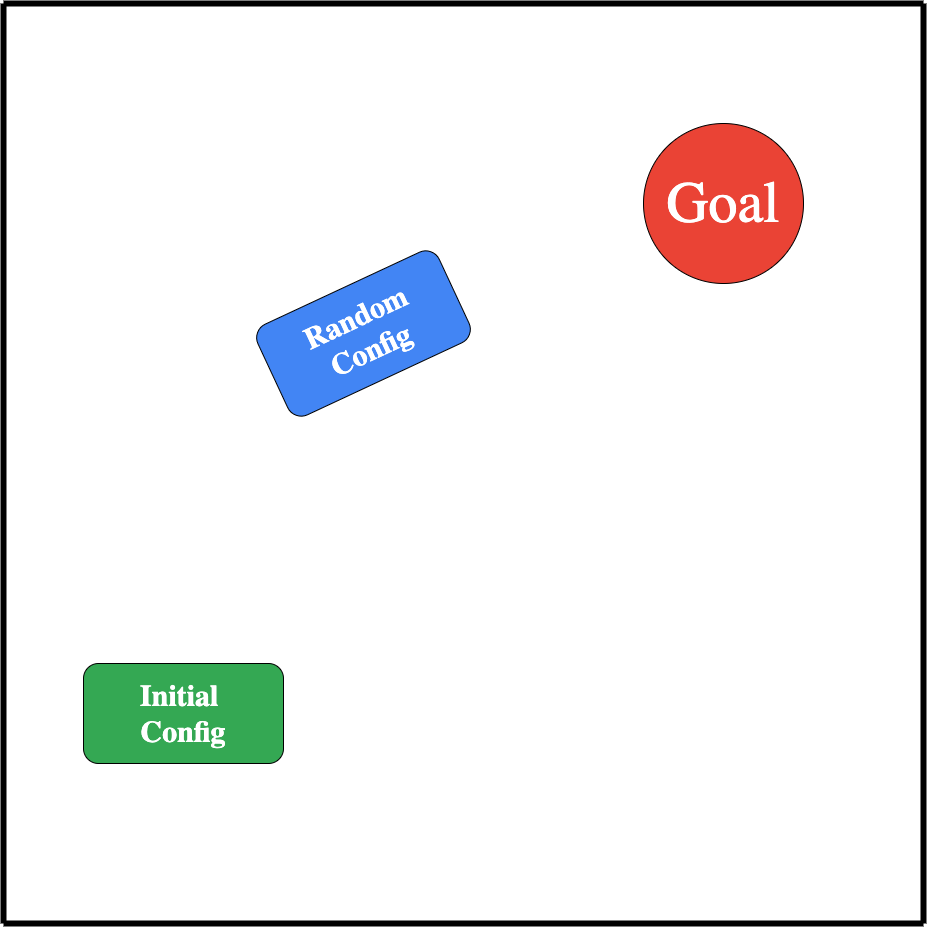
\includegraphics[width=\linewidth]{chapters/chapter2/img/RRT_step_by_step-B.png}
    \caption{The first random \gls{configuration}, $q_{rand}$, is generated}
    \label{subfig:rrt-step-by-step-B}
    \end{subfigure} \\

    % Subfigure C
    \begin{subfigure}{0.45\textwidth}
    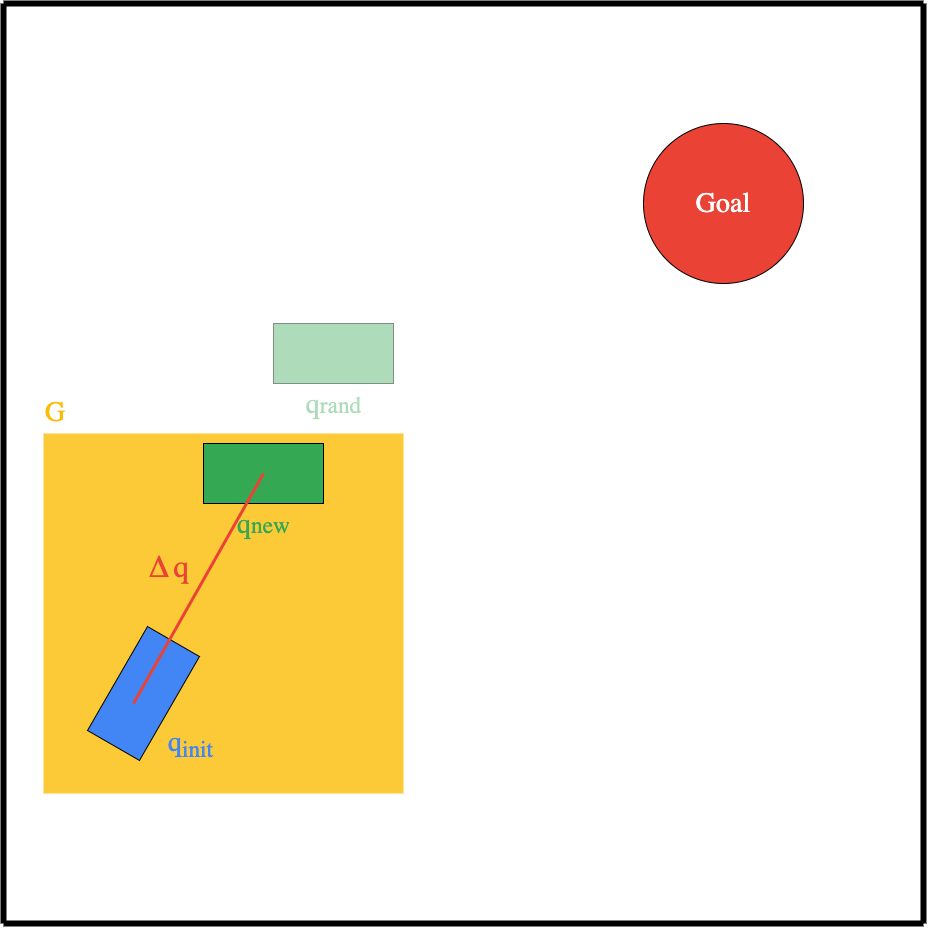
\includegraphics[width=\linewidth]{chapters/chapter2/img/RRT_step_by_step-C.png}
    \caption{In first iteration, $q_{near} = q_{init}$. Distance between $q_{init}$ and $q_{rand}$ is greater than $\Delta q$, so $q_{new}$ is generated and added to $G$}
    \label{subfig:rrt-step-by-step-C}
    \end{subfigure} &
    % 
    % Subfigure D
    \begin{subfigure}{0.45\textwidth}
    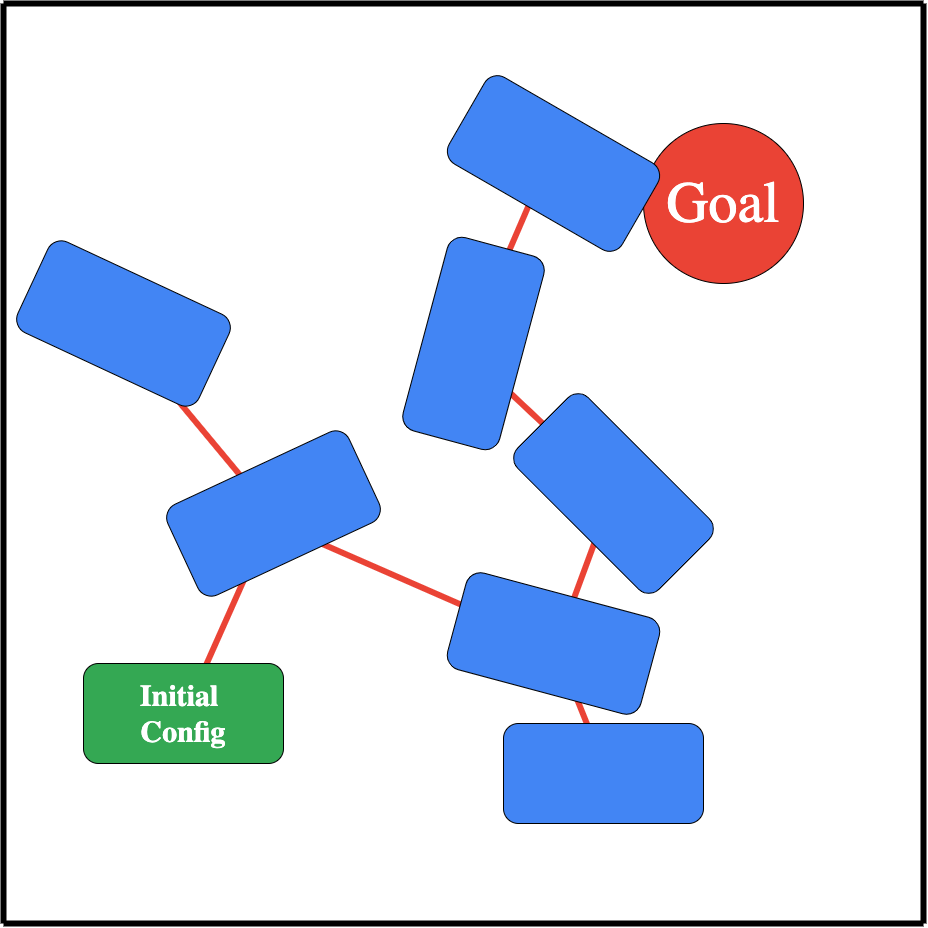
\includegraphics[width=\linewidth]{chapters/chapter2/img/RRT_step_by_step-D.png}
    \caption{This is repeated $K$ times. For $G$, $K=10$, and the red line represents the edges between \gls{configuration}s}
    \label{subfig:rrt-step-by-step-D}
    \end{subfigure}

\end{tabular}
    
    % Caption and Label
    \caption{Step by step demonstration of \gls{RRT} Algorithm for 2D robot in 2D space}
    \label{fig:rrt-step-by-step}
\end{center}
\end{figure}